\tolerance = 1600

\begin{center}
\textbf{\Large Симметрия}\\
\textit{14.07.16}
\end{center}

\epigraph{\it Неочевидное, \\ Невероятное, \\ Но явно что-то неземной красоты...}{Л. Агутин, ``Мир зелёного цвета''}

\begin{problems}
\item Внутри острого угла с вершиной $O$ взяли произвольную точку $A$. Её отразили относительно сторон угла и получили точки $A_1$ и $A_2$. Докажите, что угол $A_1OA_2$ не зависит от выбора точки.

\item а) Точки $A$ и $B$ лежат по одну сторону от прямой. Постройте на этой прямой такую точку $M$, чтобы отрезки $AM$ и $BM$ образовывали с данной прямой равные углы.

б) То же самое, но $A$ и $B$ должны лежать по разные стороны от прямой.

\begin{center}
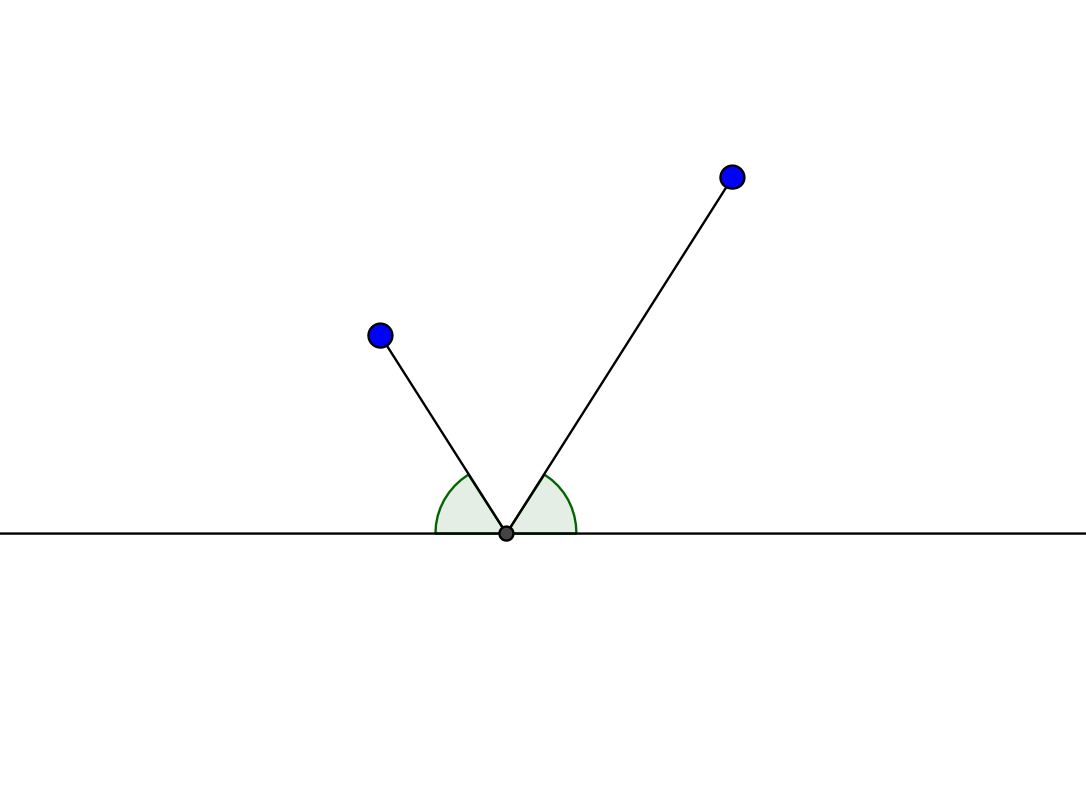
\includegraphics[width=.35\textwidth]{simm01}
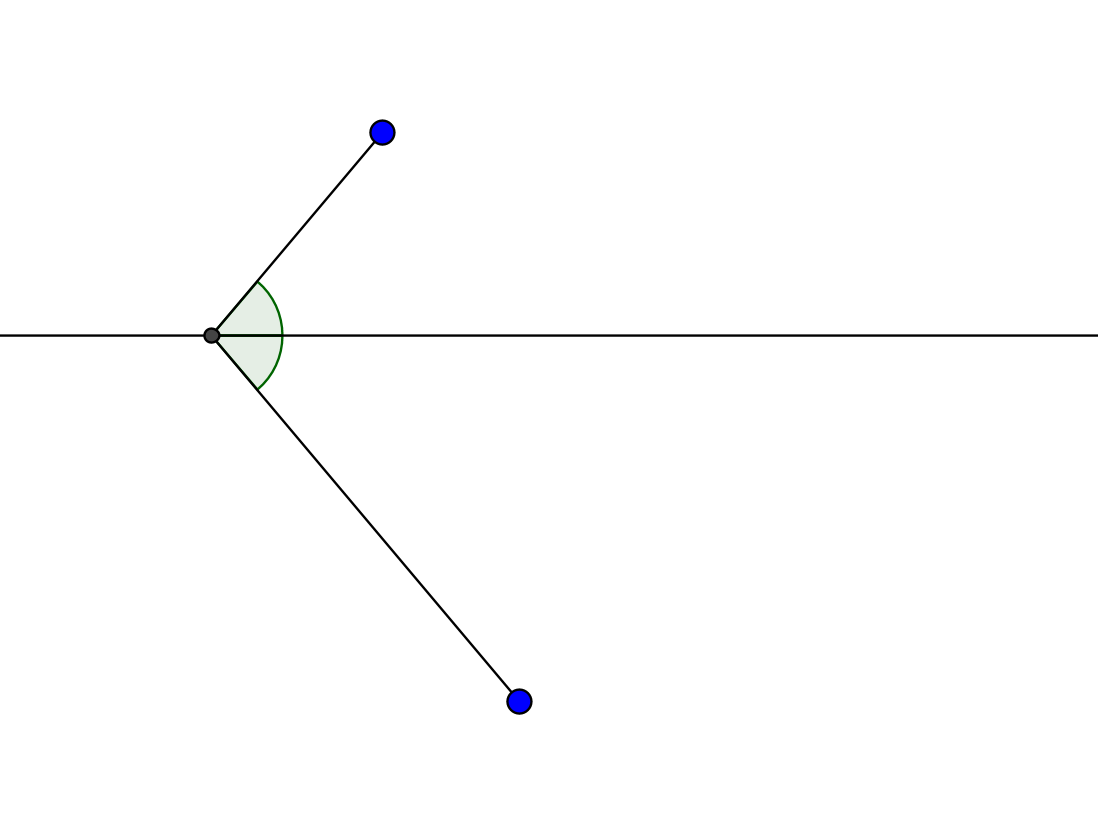
\includegraphics[width=.35\textwidth]{simm02}
\end{center}

\item а) В выпуклом четырёхугольнике $ABCD$ угол $A = 30^\circ$.

Докажите, что ${AC \leqslant BC + CD + DB}$.

б) В выпуклом четырёхугольнике $ABCD$ угол $A$ прямой.

Докажите, что ${2AC \leqslant BC + CD + DB}$.

\item Точка $M$~--- середина гипотенузы $AB$ прямоугольного треугольника $ABC$, угол $B$ которого равен $30^\circ$. На его катете $BC$ выбирают такую точку $K$, что $AK + KM = BC$. Докажите, что $MK\perp AB$.

\item На гипотенузе $AB$ и катете $BC$ прямоугольного равнобедренного треугольника $ABC$ соответственно взяли произвольные точки $M$ и $K$. Докажите, что $AK + KM \geqslant AB$.

%\item Из точки, лежащей на диаметре полукруга, под равными к нему углами провели два отрезка так, как показано на рисунке. Докажите, что сумма этих отрезков не больше диаметра полукруга.

\item На стороне $BC$ треугольника $ABC$ выбрана точка $D$. Кроме этого $$\angle{BAC}:\angle{ADC}:\angle{BCA}=3:2:1.$$ 
При этом $BC=19, AB=13$. Найдите $AD$.

\item В прямоугольнике $ABCD$ точка $M$~--- середина стороны $BC$, точка $N$~--- середина стороны $CD$, $P$~--- точка пересечения отрезков $DM$ и $BN$. Докажите, что угол $MAN$ равен углу $BPM$.

\item Биссектриса $AE$ равнобедренного треугольника $ABC$ ($AB = BC$) пересекает биссектрису его угла $B$ в точке $O$. На боковой стороне $AB$ взяли точку $M$ так, что $AM = AC$. Прямая $MO$ пересекает основание $AC$ в точке $K$. Докажите, что $AK = EC$.

%\item Внутри треугольника взяли произвольную точку. Всегда ли можно провести через неё три прямые так, чтобы отрезок каждой из них внутри треугольника делился данной точкой пополам?

\end{problems}
